\documentclass[11pt]{article}

\usepackage[margin=1in]{geometry}
\usepackage[T1]{fontenc}
\usepackage{lmodern}
\usepackage{booktabs}
\usepackage{enumitem}
\usepackage{xcolor}
\usepackage{hyperref}
\usepackage{graphicx}
\usepackage{placeins}
\usepackage{tikz}
\usepackage{pgfplots}
\usetikzlibrary{arrows.meta,positioning,shapes.geometric}
\pgfplotsset{compat=1.18}
\hypersetup{
  colorlinks=true,
  linkcolor=blue!60!black,
  urlcolor=blue!60!black,
  pdftitle={C++ UNIX File Indexer},
  pdfauthor={Project Report}
}

\title{\textbf{C++ UNIX/Linux File Indexer}\\
\large Systems Architecture, Reliability, and Performance Report}
\author{Project report}
\date{17 August 2026}

\begin{document}
\flushbottom
\maketitle

\begin{abstract}
This report documents a C++17 file indexer evolved into a UNIX/Linux systems
project without changing its word-count, Top-K, or version-difference query
semantics. The implementation combines POSIX file I/O, optional memory-mapped
input, a bounded producer--consumer pipeline, worker-local indexing, optional
process isolation with pipe IPC, and crash-safe persistent versions. The design
prioritizes correct token handling at chunk boundaries, bounded in-flight work,
and recoverable persistence. Benchmarks on a warmed 64 MiB synthetic log show
that \texttt{mmap} is modestly faster than \texttt{read()} in the single-worker
case and that worker-local indexing scales to 4.80x at eight workers.
\end{abstract}

\tableofcontents

\section{Project Goal and Scope}

The original project indexed large text/log files using a fixed-size buffer and
answered three queries:

\begin{itemize}[noitemsep]
  \item case-insensitive word-frequency lookup;
  \item Top-K word-frequency queries; and
  \item a word-frequency difference between two named versions.
\end{itemize}

The systems upgrade retained those observable semantics while adding operating
system concepts where they improve the implementation:

\begin{itemize}[noitemsep]
  \item POSIX \texttt{open()}, \texttt{read()}, \texttt{write()}, \texttt{close()},
        \texttt{fsync()}, and \texttt{rename()};
  \item optional \texttt{mmap()} input with \texttt{munmap()} cleanup;
  \item a mutex/condition-variable bounded queue;
  \item parsing and local index construction on multiple \texttt{std::thread}s;
  \item \texttt{fork()}, \texttt{exec()}, \texttt{pipe()}, and \texttt{waitpid()}
        for optional process-isolated indexing; and
  \item durable, version-addressed index files.
\end{itemize}

No external runtime dependency was added. The repository provides a
\texttt{Makefile}, test executables, and shell benchmark scripts.

\section{Architecture}

\begin{center}
\resizebox{\textwidth}{!}{%
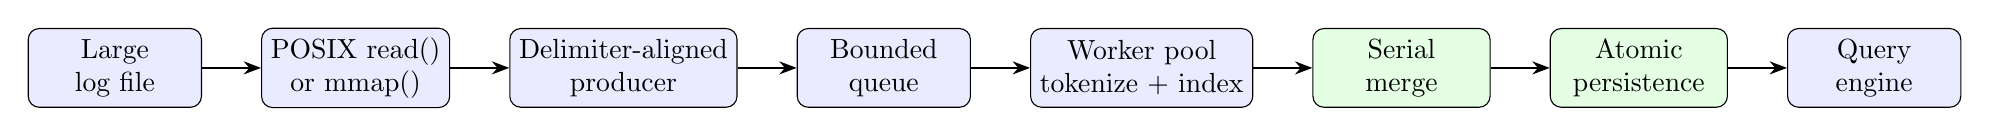
\begin{tikzpicture}[
  node distance=0.75cm,
  component/.style={draw, rounded corners, fill=blue!8, minimum width=2.2cm,
                    minimum height=1.0cm, align=center},
  store/.style={draw, rounded corners, fill=green!10, minimum width=2.25cm,
                minimum height=1.0cm, align=center},
  arrow/.style={-{Stealth[length=2.2mm]}, thick}
]
  \node[component] (input) {Large\\log file};
  \node[component, right=of input] (reader) {POSIX read()\\or mmap()};
  \node[component, right=of reader] (producer) {Delimiter-aligned\\producer};
  \node[component, right=of producer] (queue) {Bounded\\queue};
  \node[component, right=of queue] (workers) {Worker pool\\tokenize + index};
  \node[store, right=of workers] (merge) {Serial\\merge};
  \node[store, right=of merge] (persistent) {Atomic\\persistence};
  \node[component, right=of persistent] (query) {Query\\engine};

  \draw[arrow] (input) -- (reader);
  \draw[arrow] (reader) -- (producer);
  \draw[arrow] (producer) -- (queue);
  \draw[arrow] (queue) -- (workers);
  \draw[arrow] (workers) -- (merge);
  \draw[arrow] (merge) -- (persistent);
  \draw[arrow] (persistent) -- (query);
\end{tikzpicture}
}
\end{center}

The default path runs in one process. With \texttt{--process-indexer}, the
parent remains the query process and starts a child per version build. The child
executes the same binary in an internal export mode, and the completed
\texttt{WordIndex} is transferred over a pipe using a fixed-width binary
protocol. This optional mode improves fault isolation and establishes a
service-like boundary; it is not intended to maximize throughput because a
complete index must be serialized.

\paragraph{Pipeline invariants.}
Chunks are emitted only at token delimiters, the queue bounds in-flight work,
workers never share mutable frequency maps, and a version is visible on disk
only after its atomic persistence transaction completes. These invariants
connect correctness, backpressure, concurrency, and crash recovery in one
end-to-end flow.

\section{Input and Token Correctness}

\subsection{POSIX buffered I/O}

\texttt{BufferedFileReader} owns a file descriptor and a 256 KiB--1 MiB
buffer. It retries \texttt{read()} when interrupted by \texttt{EINTR}, reports
errors through exceptions, and closes the descriptor through RAII cleanup.
This replaces stream I/O while preserving the original chunk API used by the
tokenizer.

\subsection{Memory-mapped alternative}

The \texttt{mmap} reader validates that its input is a regular file, maps it
privately with \texttt{PROT\_READ | MAP\_PRIVATE}, and presents the mapping in
the same configured chunk sizes. It therefore changes the transport mechanism,
not tokenization or query semantics. Empty files are handled without calling
\texttt{mmap()} with a zero length.

\subsection{Boundary-safe parallel work}

Tokenization treats contiguous alphanumeric bytes as one lower-cased word.
Independent workers cannot safely tokenize arbitrary byte chunks because a word
can span a chunk boundary. The producer solves this by retaining an unfinished
suffix and emitting work only through the most recent non-alphanumeric
delimiter. Every queued chunk is therefore independently tokenizable. The
final suffix is flushed at end of file.

This scheme keeps queued work bounded in count. Extremely long individual words
can still make the producer's retained suffix grow, which is required to
preserve exact word semantics and is a documented edge case rather than a
hidden truncation.

\section{Concurrency and Synchronization}

\subsection{Bounded producer--consumer queue}

\texttt{BoundedBlockingQueue<T>} is a multi-producer, multi-consumer queue
with a fixed capacity of eight chunks in the indexing pipeline. A mutex guards
the deque and closed state. Two condition variables express the exact blocking
conditions:

\begin{itemize}[noitemsep]
  \item \texttt{notFull}: producers wait while the queue is full;
  \item \texttt{notEmpty}: consumers wait while the queue is empty; and
  \item \texttt{close()}: wakes both sides, rejects future pushes, and lets
        consumers drain already queued work.
\end{itemize}

Using condition variables is preferable to adding semaphores here because the
queue needs both a capacity predicate and a drain-after-close predicate.

\subsection{Index ownership model}

Each worker owns one private \texttt{WordIndex}; no worker mutates another
worker's hash map. After all threads join, the caller merges the local maps
serially. This removes a shared hash-map mutex from the hot token-update path.
The queue and the worker exception pointer are the only shared mutable states,
and both are synchronized. Thread joins establish the happens-before boundary
before the merge.

\section{Process Isolation and IPC}

\texttt{--process-indexer} creates a unidirectional pipe, forks, redirects the
child's standard output to the pipe, then execs the same executable with an
internal index-export flag. The parent reads and validates:

\begin{enumerate}[noitemsep]
  \item a protocol magic value;
  \item the number of entries;
  \item each fixed-width word length, word bytes, and signed frequency.
\end{enumerate}

Partial reads and writes, including \texttt{EINTR}, are handled explicitly.
The parent closes the pipe and uses \texttt{waitpid()} to reject signaled or
nonzero-exit children. This avoids treating an incomplete IPC transfer as a
valid index.

\section{Crash-Safe Persistent Versions}

Passing \texttt{--index-dir PATH} saves every newly built version. The
persistence transaction is:

\begin{enumerate}[noitemsep]
  \item create a unique temporary file in the destination directory;
  \item serialize the index and \texttt{fsync()} the temporary file;
  \item close it and atomically replace the target using \texttt{rename()};
  \item on Linux, \texttt{fsync()} the containing directory to make the rename
        durable; and
  \item remove the temporary file if a pre-rename step fails.
\end{enumerate}

The target name is derived from a hex encoding of the logical version name, so
version names cannot traverse out of the configured directory. Loading is
explicit through \texttt{--load-index}; the program never substitutes a
persisted version for a requested source file without the user's instruction.

\section{CLI and Reproducibility}

\begin{verbatim}
make
make test

./build/file-indexer --query word --reader mmap --workers 4 \
  --file data/log.txt --version v1 --buffer 1024 --word error

./build/file-indexer --query word --file data/log.txt --version v1 \
  --buffer 1024 --index-dir indexes --word error
./build/file-indexer --query word --load-index --index-dir indexes \
  --version v1 --word error
\end{verbatim}

\texttt{make test} builds and executes four focused tests:

\begin{itemize}[noitemsep]
  \item bounded-queue backpressure, closure, and multi-producer/multi-consumer
        behavior;
  \item a word deliberately crossing a 256 KiB input boundary with both
        \texttt{read} and \texttt{mmap} modes;
  \item index serialization round-trip and invalid-frequency rejection; and
  \item persistent save, load, and atomic replacement.
\end{itemize}

\section{Benchmark Methodology}

All reported benchmarks use a warmed, 64 MiB synthetic text log containing
repeating alphanumeric words, a 1 MiB chunk size, and three iterations. The
workload is deliberately simple and should not be treated as a universal
production result. It is useful for comparing implementation modes under the
same conditions.

Latency is the application's reported complete index-build time. Throughput is
computed as input bytes divided by average latency. The benchmark invokes a
missing-word query, ensuring that every run builds the full index. Peak-memory
measurement is supplied by \texttt{benchmark\_memory.sh}: it uses
\texttt{/usr/bin/time -l} on macOS and \texttt{/usr/bin/time -v} on Linux.
Restricted environments may deny access to memory counters; the script reports
that condition rather than inventing a value.

\section{Benchmark Results}

\subsection{Reader mode comparison}

\begin{table}[ht]
\centering
\caption{Single-worker reader benchmark, warmed 64 MiB input. Lower latency and
higher throughput are better.}
\begin{tabular}{lrr}
\toprule
Reader & Average latency (s) & Throughput (MiB/s) \\
\midrule
\texttt{read()} & 0.24233 & 264.10 \\
\texttt{mmap()} & 0.22633 & 282.77 \\
\bottomrule
\end{tabular}
\end{table}

\begin{figure}[ht]
\centering
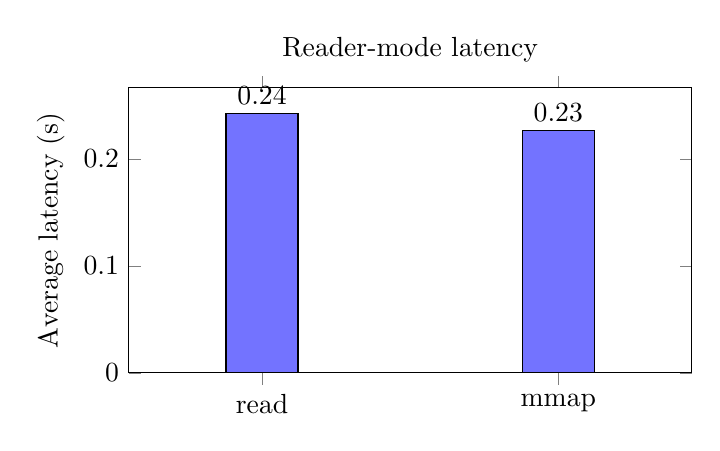
\begin{tikzpicture}
\begin{axis}[
  ybar,
  bar width=26pt,
  width=0.72\linewidth,
  height=5.2cm,
  ymin=0,
  ylabel={Average latency (s)},
  symbolic x coords={read,mmap},
  xtick=data,
  nodes near coords,
  nodes near coords align={vertical},
  enlarge x limits=0.45,
  title={Reader-mode latency}
]
\addplot[fill=blue!55] coordinates {(read,0.24233) (mmap,0.22633)};
\end{axis}
\end{tikzpicture}
\caption{The \texttt{mmap} mode was about 6.6\% faster in this warmed,
single-worker workload.}
\end{figure}
\FloatBarrier

\subsection{Worker scaling with \texttt{mmap}}

\begin{table}[ht]
\centering
\caption{\texttt{mmap} scaling benchmark, warmed 64 MiB input.}
\begin{tabular}{rrrr}
\toprule
Workers & Average latency (s) & Throughput (MiB/s) & Speedup \\
\midrule
1 & 0.22512 & 284.29 & 1.00x \\
2 & 0.11830 & 541.00 & 1.90x \\
4 & 0.07030 & 910.38 & 3.20x \\
8 & 0.04689 & 1364.90 & 4.80x \\
\bottomrule
\end{tabular}
\end{table}

\begin{figure}[ht]
\centering
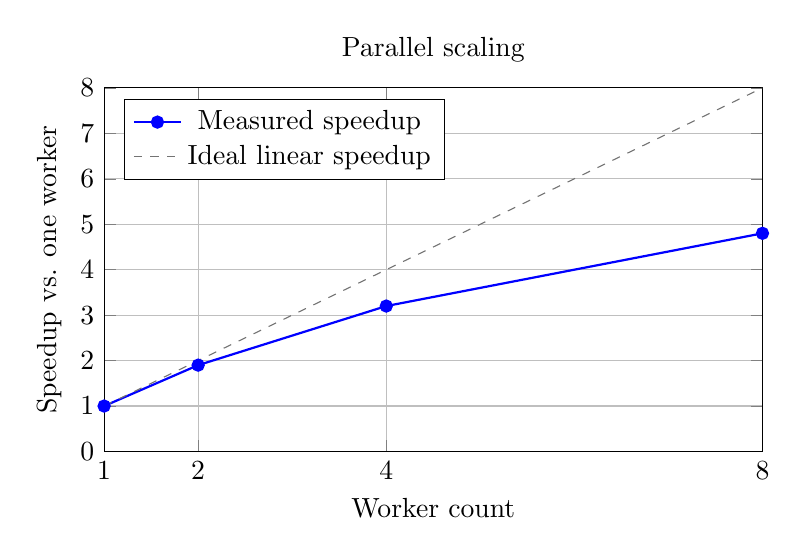
\begin{tikzpicture}
\begin{axis}[
  width=0.82\linewidth,
  height=6.2cm,
  xlabel={Worker count},
  ylabel={Speedup vs. one worker},
  xmin=1, xmax=8,
  ymin=0, ymax=8,
  xtick={1,2,4,8},
  ytick={0,1,2,3,4,5,6,7,8},
  grid=both,
  legend style={at={(0.03,0.97)}, anchor=north west},
  title={Parallel scaling}
]
\addplot[blue, mark=*, thick] coordinates {
  (1,1.00) (2,1.90) (4,3.20) (8,4.80)
};
\addlegendentry{Measured speedup}
\addplot[black!55, dashed, domain=1:8, samples=100] {x};
\addlegendentry{Ideal linear speedup}
\end{axis}
\end{tikzpicture}
\caption{Scaling is strong but sublinear. At eight workers, the serial producer,
memory subsystem, and final merge increasingly limit throughput.}
\end{figure}
\FloatBarrier
\section{Interpretation and Bottlenecks}

The measurements show three useful conclusions:

\begin{enumerate}
  \item \textbf{Reader choice matters, but not alone.} The warmed \texttt{mmap}
        advantage was small because tokenization and hash-map updates dominate
        much of the end-to-end work.
  \item \textbf{Worker-local maps scale well.} Removing a shared-map mutex lets
        workers process different delimiter-aligned chunks with little
        contention at low and moderate worker counts.
  \item \textbf{Amdahl's law remains visible.} The producer is single-threaded,
        and the final map merge is serial. These portions, together with memory
        bandwidth, explain the gap between 4.80x measured and 8x ideal speedup.
\end{enumerate}

Expected bottlenecks on more diverse workloads are:

\begin{itemize}[noitemsep]
  \item producer delimiter scanning and queue coordination at high worker counts;
  \item allocation, lowercasing, and hashing for high-cardinality vocabularies;
  \item page faults and storage bandwidth on cold data;
  \item final local-map merge cost for many unique words;
  \item complete-index pipe serialization in process-isolated mode; and
  \item synchronous file and directory durability work for persistent versions.
\end{itemize}

For a production evaluation, record CPU model, available memory, compiler,
operating system, storage medium, reader mode, chunk size, worker count, file
size, token distribution, and whether the page cache was cold or warm. Cold-I/O
tests and warmed CPU-scaling tests answer different questions and should be
reported separately.

\section{Conclusion}

The project is now a complete systems-oriented file indexer. Its core query
semantics remain simple, while its implementation demonstrates practical UNIX
techniques: descriptor-based I/O, memory mapping, bounded synchronization,
multithreading, process boundaries, binary pipe IPC, and crash-safe
persistence. The implementation favors explicit tradeoffs over resume-driven
features: process mode is optional because it costs serialization time, and
worker-local indexes avoid a shared-map lock because that lock would degrade
the hot path. The included tests, Makefile, and benchmark scripts make those
choices reproducible and measurable.

\end{document}
